
%% put the key last to have correct numbering

\begin{figure*}

\centering
  \vspace*{0.3in}
 \subfloat[10GbE: Multi-core scalability (n=1;s=64B)]{
  \label{fig:short10:mcore}
   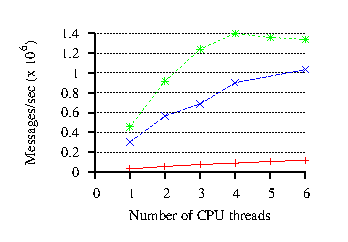
\includegraphics{figs/short-mcore10.eps}}
 \hspace{.01in}
 \subfloat[10GbE: $n$ roundtrips per conn. (s=64B)]{
  \label{fig:short10:roundtrips}
  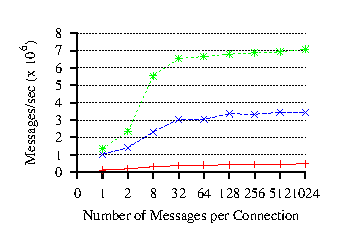
\includegraphics{figs/short-roundtrips10.eps}}
  \hspace{.01in}
 \subfloat[10xGbE: Different message sizes $s$ (n=1)]{
  \label{fig:short10:size}
  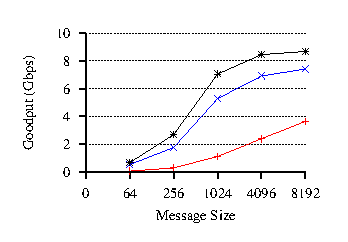
\includegraphics{figs/short-size10.eps}}
 \centering

 \centering
 \vspace*{0.1in}
 \subfloat[4x10: Multi-core scalability (n=1;s=64B)]{
  \label{fig:short40:mcore}
   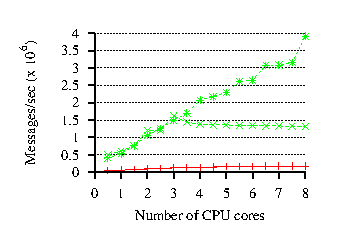
\includegraphics{figs/short-mcore40.eps}}
 \hspace{.01in}
 \subfloat[4x10: $n$ roundtrips per conn. (s=64B)]{
  \label{fig:short40:roundtrips}
  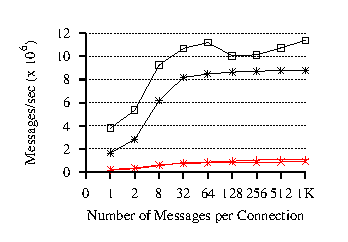
\includegraphics{figs/short-roundtrips40.eps}}
  \hspace{.01in}
 \subfloat[4x10: Different message sizes $s$ (n=1)]{
  \label{fig:short40:size}
  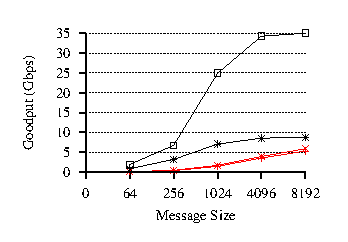
\includegraphics{figs/short-size40.eps}}

  \vspace{-3.8in}
  \subfloat{
\includegraphics{figs/short-key10.eps}}
 \vspace{1.3in}
 \centering \subfloat{
\includegraphics{figs/short-key40.eps}}
 \vspace{1.5in}


\caption{Short message performance on the 10GbE and 4x10GbE setups.}
 \label{fig:shortboth}

\end{figure*}
